\newpage
\section{Farkas-lemma (két alakban), a lineáris program célfüggvény korlátossága}

A következő egyenletekből csak a jobb vagy csak a bal egyenletrendszereknek
létezik egyidőben megoldása (a Farkas~\footnote{Farkas Gyula, 1902.} lemma két
alakja):

\begin{enumerate}
  \item alak: \begin{align*}
  \overbrace{Ax \leq b}^{A1}  && \overbrace{yA= 0}^{A2}\\
   			 && y\geq 0 \\
             && yb< 0
  \end{align*}
  \item alak:\begin{align*}
  \overbrace{Ax = b }^{B1}   && \overbrace{yA \geq 0}^{B2}\\
  x \geq 0 && yb < 0 
  \end{align*}
\end{enumerate}

Legyen az alábbi mérettel rendelkező mátrixok:
\[
\overbrace{\begin{bmatrix} 1 &  \cdots &  n \end{bmatrix}}^{\hbox{y}} 
\overbrace{\begin{bmatrix} 1 & \cdots & n \\ \vdots & \ddots & \vdots \\ m  & \cdots & 0 \end{bmatrix}}^{\hbox{A}}
\underbrace{\begin{bmatrix} 1 \\ \vdots \\  n \end{bmatrix}}_{\hbox{x}}
\overbrace{\begin{bmatrix} 1 \\ \vdots \\  m \end{bmatrix}}^{\hbox{b}}.
\]

\subsection{1--es alak}
Az első alak két egyenletrendszere nem megoldható egyidőben mert:
\[ 0 = 0x = (yA) \cdot x = y(Ax) \leq yb.\] Az átcsoportositást megtehetjük a
szorzás asszociativitása miatt, míg az utolsó egyenlőtlenséget is át kell
gondolni: \[ Ax \leq b \Rightarrow y(Ax) \leq yb.\] Szerencsére ez igaz lesz
mivel $Ax$ elemei legyenek $\alpha_i$, $b$ elemei $\beta_i$ és $y$ elemei
$\gamma_i$.
$\sum\gamma_i \alpha_i \leq \sum \gamma_i \beta_i \Rightarrow y(Ax) \leq y(b)$,
mivel adott $y \geq 0$ feltétel (tehát $\gamma_i \geq 0$). Majd tovább futtatva a
korábbi gondolatunkat $yb<0$ amely ellentmond a kiinduló feltételeknek ($0=yAx \leq yb<0$). 

Vizsgáljuk meg, hogy mi történik, ha $A1$ nem megoldható (ezt tegyük fel),
következik e ebből, hogy az $A2$ igen? Definiáljuk a következő $C$ halmazt,
amely egy sorvektorok halmaza, és az $A2$ alak egyenleteire épül: \[ C= \left\{
z \in \mathbb{R}^{n+1} | z = y (A|b), y \geq 0 \right\}\].

Célunk bizonyítani, hogy létezik $C$-ben $(0, \cdots, 0 , <0)$ alakú sorvektor
(ez azt jelentené, hogy az $A2$--nek létezzik egy $y$ megoldása), ha az $A1$
($Ax \leq b$) egyenletrendszer nem megoldható.A megoldáshoz indukciót
használunk, felhasználva a Fourier--Motzkin eliminációt. Lássuk be, hogy az
elimináció során felhasznált műveletek (szorzás pozítiv skalárral és vektorok
összeadása) nem vezetnek ki a halmazból.

A halmaz zártságára az alábbi lemmák igazak ($z_1, z_2 \in C, \lambda>0$):

\begin{itemize}
  \item $z_1+z_2 \in C$, mert $\begin{rcases}
  z_1=y_1(A|b) \\
  z_2=y_2(A|b) \end{rcases} \Rightarrow z_1+z_2=(y_1+y_2)(A|b)$ ahol $y_1+y_2 \geq 0,$
  \item $\lambda z_1 \in C$, mert $
  z=y(A|b) \Rightarrow \lambda z = \lambda y (A|b)$ ahol igaz, hogy $\lambda y \geq 0$.
\end{itemize}

Bizonyitjuk, hogy az eliminációval párhuzamosan mindig létre tudunk hozni ilyen
elemet a $C$--ben, ha $A1$--nek nincs megoldása (mint a kezdeti halmaz elemek
egy lineáris kombinációja). Kiindulunk kezdeti $(A|b)$ mátrixból, amely sorai
$\in C$, mert $y_i=1$--el (máshol a vektor $0$) felvételt nyernek $C$--be. Most
hajtsuk végre a Fourier-Motzkin eliminációt $(A|b)$--re, úgy, hogy a nullákat
nem töröljük:

\begin{displaymath}
\underbrace{
\begin{array}{|cccc|c|}
\hline
 &  &  &  & \\
 &  & &  & \\
A &  & &  &b \\
 &  & & &\\
\hline
\end{array}}_{\mbox{sorai } \in~C}
\Rightarrow
\underbrace{
\begin{array}{|c|ccc|c|}
\hline
0 &  &  &  & \\
\hline
0 &  & &  & \\
0 &  & &  & \\
\hline
0 &  & & &\\
\hline
\end{array}}_{\mbox{sorai } \in~C}
\Rightarrow
\underbrace{
\begin{array}{|ccc|c|c|}
\hline
0 &  0 &0  & +1  & b_+\\
\hline
0 &  0& 0&  -1& b_-\\
\hline
0 &  0& 0& 0& b_0\\
\hline
\end{array}}_{\mbox{sorai } \in~C}
\end{displaymath}

A zártsági lemma miatt az elimináció során a mátrix sorai $C$ halmazon belül
maradnak. Végezzük el az eliminációt ismét és ismét amíg egy változós alakra nem
jutunk. Ha a feladat eredetileg nem volt megoldható, ezt a tulajdonságot az
elimináció megtartja, a végén sem lesz az, ez meg két feltétel melett történhet meg:

\begin{itemize}
  \item Létezik $0 \cdot x_n \leq \gamma$ egyenlet, ahol $\gamma < 0$. Ennek alakja 
  $(0,0, \cdots, 0, <0),$ tehát a sor $\in C$.
  \item $\begin{rcases}
  +1 \cdot x_n \leq \alpha_i \\ 
  -1 \cdot x_n \leq \alpha_j \\
  \end{rcases} \Rightarrow  \mbox{ ellentmondáshoz meg akkor jutunk ha }
  \alpha_i < -\alpha_j.$
  
  Az $i$ sor alakja $(0, \cdots, 0, +1, \alpha_i)$, a $j$ sor meg $(0, \cdots,
  0, -1, \alpha_j)$. Ennek az összege meg $(0, \cdots, 0, 0, \alpha_i+\alpha_j)$
  ami szintén $\in C$, mivel $\alpha_i+\alpha_j<0$.
\end{itemize}

\subsection{2--es alak}

Az, hogy a két egyenletrendszer ($B1$ és $B2$) közül csak az egyik megoldható
egy időben indirekt bizonyítjuk. Legyen $x,y$ egy--egy megoldás:

\[ 0 \leq \underbrace{
		   \underbrace{(yA)}_{\mbox{sorvektor}}x = 
		  y\underbrace{(Ax)}_{\mbox{oszlopvektor}}}
		  _{\mbox{nem triviális lépés}}=yb<0\] ahol ellentmondáshoz jutunk.

Az hogy ha az egyik nem megoldható a másik igen visszavezetéssel bizonyítjuk az
$1$--es alakra. Ehhez először is kibontjuk a $B1$ alakot:
\[ 
\begin{rcases}
Ax =b \\
x \geq 0
\end{rcases} \Rightarrow
\begin{cases}
A x    &\leq b \\
(-A x) &\leq -b \\
(-E x) &\leq 0
\end{cases}
\]
Most ennek az $A1$ alaknak felírjuk $B1$ alakját mint: 

\begin{displaymath}
\begin{array}{|c|c|c|}
\hline
A \\ \hline
-A \\ \hline
-E\\  \hline
\end{array}
~ x\leq
\begin{array}{|c|c|c|}
\hline
0 \\ \hline
0 \\ \hline
0  \\  \hline
\end{array}
\Rightarrow
\underbrace{
\begin{array}{|c|c|c|}
\hline
y_1 & y_2  & y_3\\
\hline
\end{array}}_{y'}
\underbrace{
\begin{array}{|c|}
\hline
A \\
\hline
-A\\
\hline
-I \\
\hline
\end{array}}_{A'}
=0,~
\begin{array}{|c|}
\hline
y_1\\\hline
y_2\\\hline
y_3\\
\hline
\end{array}^T
\geq
\begin{array}{|c|}
\hline
0\\\hline
0\\\hline
0\\
\hline
\end{array}^T,~
~
\begin{array}{|c|c|c|}
\hline
y_1&
y_2&
y_3 \\
\hline
\end{array}
~
\begin{array}{|c|}
\hline
b\\\hline
-b\\\hline
0\\
\hline
\end{array}
<0
\end{displaymath}

Azt állítjuk, hogy ha ez nem megoldható, akkor a $ yA \geq 0$, $yb \leq 0$ páros
igen.

\begin{align*}
y_1 A + y_2 (-A) + y_3(-I) &= 0 \\
y_1 \cdot b - y_2 \cdot b + y_3 \cdot 0 &<0, \\
y_1, y_2, y_3 &\geq 0
\end{align*}

Tehát:
\[
\begin{rcases}
(y_1 - y_2) \cdot A &= y_3 \\ 
(y_1 - y_2) \cdot B &< 0 \\
y_1, y_2, y_3 &\geq 0
\end{rcases} \xRightarrow{y=y_1-y_2} 
\begin{cases}
y \cdot A &\geq 0 \\ 
y \cdot B &< 0
\end{cases}
\]
Ezzel felírtuk $B2$ alakot, azaz a $B1\xRightarrow{?}B2$ bizonyitását
visszavezetük $A1 \Rightarrow A2$--re.

\subsection{Korlátosság}

Az alábbi három kijelentés ekvivalens:

\begin{enumerate}
  \item $cx$ felülről korlátos az $Ax \leq b$ megoldás halmazon.
  \item $\not \exists$ megoldása az $ \begin{cases}
  Az \leq 0 \\
  cz > 0
  \end{cases} $ egyenletrendszernek.
  \item ~$\exists$ megoldása a~~$\begin{cases}
  yA=c \\
  y \geq 0
  \end{cases}$ egyenletrendszernek.
\end{enumerate}

A tétel bizonyítását \aref{fig:KorBizKor} ábra szerint fogjuk belátni.
 
\begin{figure}[htbp]
\caption{A korlátosság bizonyítási kőrre}
\label{fig:KorBizKor}
\centering 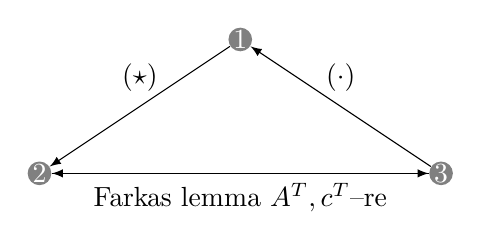
\begin{tikzpicture}[scale=1.7]
  \tikzset{ p/.style={circle,white,fill=gray,inner sep=0pt,minimum size=0.3cm},
  }
  \node[p] (1) at (0, 0) {1};
  \node[p] (2) at (-1.5, -1) {2}; 
  \node[p] (3) at (+1.5 , -1) {3};
  
  % the connection between the dots
  \draw[-latex] (1) -- (2) node [midway, above=2pt] {($\star$)}; 
  \draw[-latex] (3) -- (1) node [midway, above=2pt] {($\cdot$)}; 
  \draw[-latex] (2) -- (3) node [midway, below] {Farkas lemma $A^T,c^T$--re};
  \draw[-latex] (3) -- (2);
\end{tikzpicture} 

\newcommand*\circled[1]{\tikz[baseline=(char.base)]{
            \node[shape=circle,draw,inner sep=1pt] (char) {#1};}}
            
\begin{description}
  \item[($\star$) -- \circled{1} $\Rightarrow$ \circled{2}:]  Legyen $x_0$
  megoldása az $Ax \leq b$--nek és tegyük fel, hogy mégis létezik megoldása
  \circled{2}--nek. Ekkor legyen $\lambda > 0$, $x_0 + \lambda z$ is megoldása
  az $Ax \leq b$--nek, mert:
  \[ A(x_0+ \lambda z) = Ax_0 + \lambda (Az) \leq A x_0 + 0 \leq b \] Továbbá
  $c(x_0 + \lambda z ) = c x_0 + \lambda (cz)$, és mivel $cz>0$ a $\lambda$
  alkalmas megválasztásával ez tetszőleges naggyá tehető. Ez meg ellentmond
  \circled{1}--nek, tehát feltevésünk hamis volt.
  \item[($\cdot$) -- \circled{3} $\Rightarrow$ \circled{1}:]  Legyen egy $y$
  ami teljesíti \circled{3}--at és $x$ ami megoldása \circled{1}--nek. 
  \[ cx = (yA)x = y(Ax) \leq yb \]
  Ekkor $yb$ a keresett felső korlát az $Ax$ megoldás halmazán $cx-re$, tehát
  \circled{3}--ból következik \circled{1}.
\end{description}